\documentclass[main.tex]{subfiles}
\begin{document}

\marginpar{Tuesday\\ 2020-11-3, \\ compiled \\ \today}

\begin{figure}[ht]
\centering
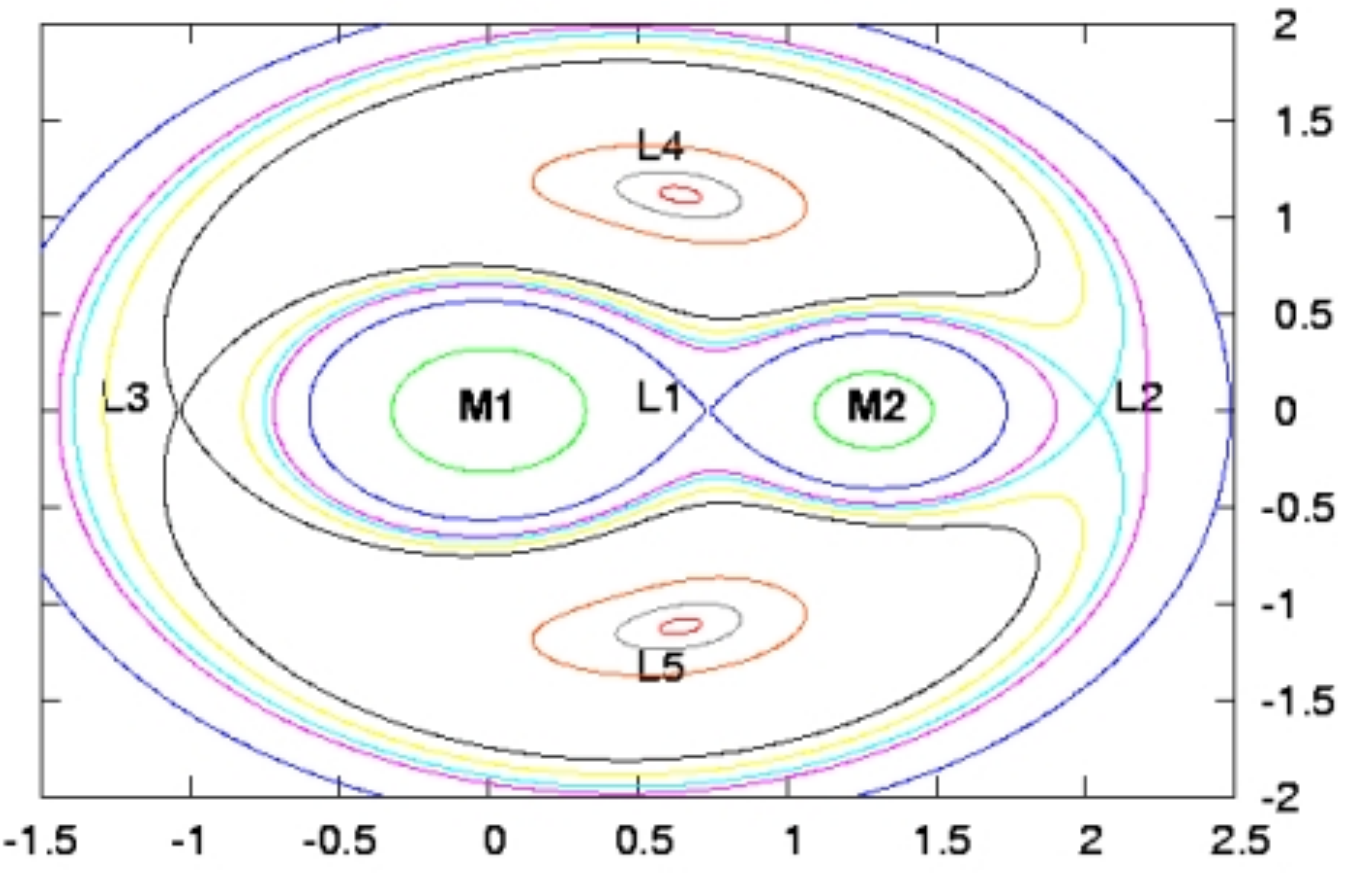
\includegraphics[width=\textwidth]{figures/roche-equipotential}
\caption{Equipotential lines for the Roche potential \(\phi _R\). \(M_{1, 2}\) mark the two masses, while the Lagrange points\(L\) are the ones in which the potential is stationary: \(\nabla \phi _R = 0\).}
\label{fig:roche-equipotential}
\end{figure}

% The equation of motion of a particle in the corotating frame is 
% %
% \begin{align}
% \pdv{\vec{v}}{t} 
% + \qty(\vec{v} \cdot \vec{\nabla}) \vec{v}
% = - \frac{1}{\rho } \vec{\nabla} P 
% - \vec{\omega} \wedge \vec{v}
% - \vec{\nabla} \phi _R
% \,,
% \end{align}
% %
% where \(\phi _R\) is the Roche potential, which can be written in terms of the parameters \(q = M_2 / M_1 \) and \(a\);
%
% \todo[inline]{there might be a wrong sign in the last lecture!} 
%
% \begin{align}
% \phi _R = - \frac{GM_1}{\abs{\vec{r} - \vec{r}_1}}
% - \frac{GM_2}{\abs{\vec{r} - \vec{r}_2}}
% - \frac{1}{2} \qty(\vec{\omega} \wedge \vec{r})^2
% \,.
% \end{align}
% \todo[inline]{insert diagram for the quantities in the potential}

Also, if \(\theta \) is the angle between \(\vec{\omega}\) and \(\vec{r}\) we can write 
%
\begin{align}
\qty(\vec{\omega} \wedge \vec{r})^2 = \omega^2 r^2 \sin^2 \theta 
\,.
\end{align}

Let us come back to the Roche potential, whose equipotential contours we sketch in figure \ref{fig:roche-equipotential}. 
In terms of the aforementioned variables \(q\) and \(\theta \) it can be written as
%
\begin{align}
\phi _R &=  
- G (M_1 + M_2 ) \qty[ + \frac{1}{2} \frac{\omega^2 r^2 \sin^2\theta }{G (M_1 + M_2 )}
+ \frac{GM_1 }{G (M_1 + M_2 ) \abs{\vec{r} - \vec{r}_1 }}
+ \frac{GM_2 }{G (M_1 + M_2 ) \abs{\vec{r} - \vec{r}_2 }}
 ]  \\
 &= - G (M_1 + M_2 )
 \qty[
     \frac{1}{2} \frac{\omega^2r^2 \sin^2\theta }{G(M_1 + M_2 )} 
     + \frac{1}{(1 + q) \abs{\vec{r} - \vec{r}_1}}
     + \frac{q}{(1 + q) \abs{\vec{r} - \vec{r}_2}}
 ]
\,.
\end{align}

We can then use Cartesian coordinates centered in \(M_1 \): 
then, 
%
\begin{align}
\phi _R = - \frac{G (M_1 + M_2  )}{2 a^3}
\qty[ \frac{2 a^3}{1 + q}
\frac{1}{\sqrt{x^2 +y^2 +z^2}}
+
\frac{2 q a^3}{1 + q} 
\frac{1}{\sqrt{(x-a)^2 + y^2 +z^2}}
+ \qty[(x - x _{\text{CM}})^2 + y^2]
]
\,,
\end{align}
%
where 
%
\begin{align}
x _{\text{CM}} = \frac{qa}{1 + q}
\,,
\end{align}
%
so if we rescale all the spatial coordinates by the major semi axis \(a\) we get 
%
\begin{align}
\phi _R = - \frac{G (M_1 + M_2 )}{2a}
\qty[
\frac{2}{1 +q}
\frac{1}{\sqrt{x^2 +y^2 +z^2}} 
+
\frac{2 q}{1 + q} 
\frac{1}{\sqrt{(x-1)^2 + y^2 + z^2}}
+ \qty[\qty(x - \frac{q}{1 + q})^2 + y^2]
]
\,.
\end{align}

If the stars are stationary, or in slow evolution. Then, their surfaces will be (at least in first approximation) at rest. Therefore, the derivative terms vanish, and we get 
%
\begin{align}
0  = - \frac{1}{\rho } \vec{\nabla} P - \vec{\nabla} \phi _R
\,,
\end{align}
%
but the surface is defined by \(\vec{\nabla} P = 0\), which by this equation corresponds to \(\vec{\nabla} \phi _R = 0\). 

The star will then take the shape of an equi-Roche potential surface. 
What is this shape? 

\todo[inline]{Make 2D plots, cuts of the surface}

\subsection{The Roche lobe}

We have roughly spherical contours near the stars, and a figure-eight contour eventually.
The center of this contour is called \(L_1 \), the first or ``inner'' Lagrange point. 

Analogy with a dog food container for Roche Lobe overflow.

Is the overflow stable? It depends on whether the volume of the Roche lobe increases or decreases as the donor star loses mass: in the latter case. 

% Tight worn jeans? 

We can introduce a characteristic \textbf{radius} of the Roche Lobe, calculated by 
%
\begin{align}
V _{\text{lobe}} = \frac{4}{3} \pi R _{\text{lobe}}^3
\,,
\end{align}
%
although the lobe is not a sphere this allows us to give a characteristic number. 
We can calculate \cite[]{eggletonApproximationsRadiiRoche1983}:
%
\begin{align}
\frac{R_{\text{lobe}}}{a} = f(q) \approx
\begin{cases}
    \num{.38} + \num{.2} \log_{10} q  & \num{.5} < q < \num{20}\\
    \num{.46}  \qty( \frac{q}{1 + q})^{1/3}
    & 0 < q < \num{.5}
\end{cases} 
\,,
\end{align}
%
and we can see that the dependence on \(q\) is quite weak. A plot of this is shown in figure \ref{fig:roche-lobe-radius}:
%
\begin{figure}[ht]
\centering
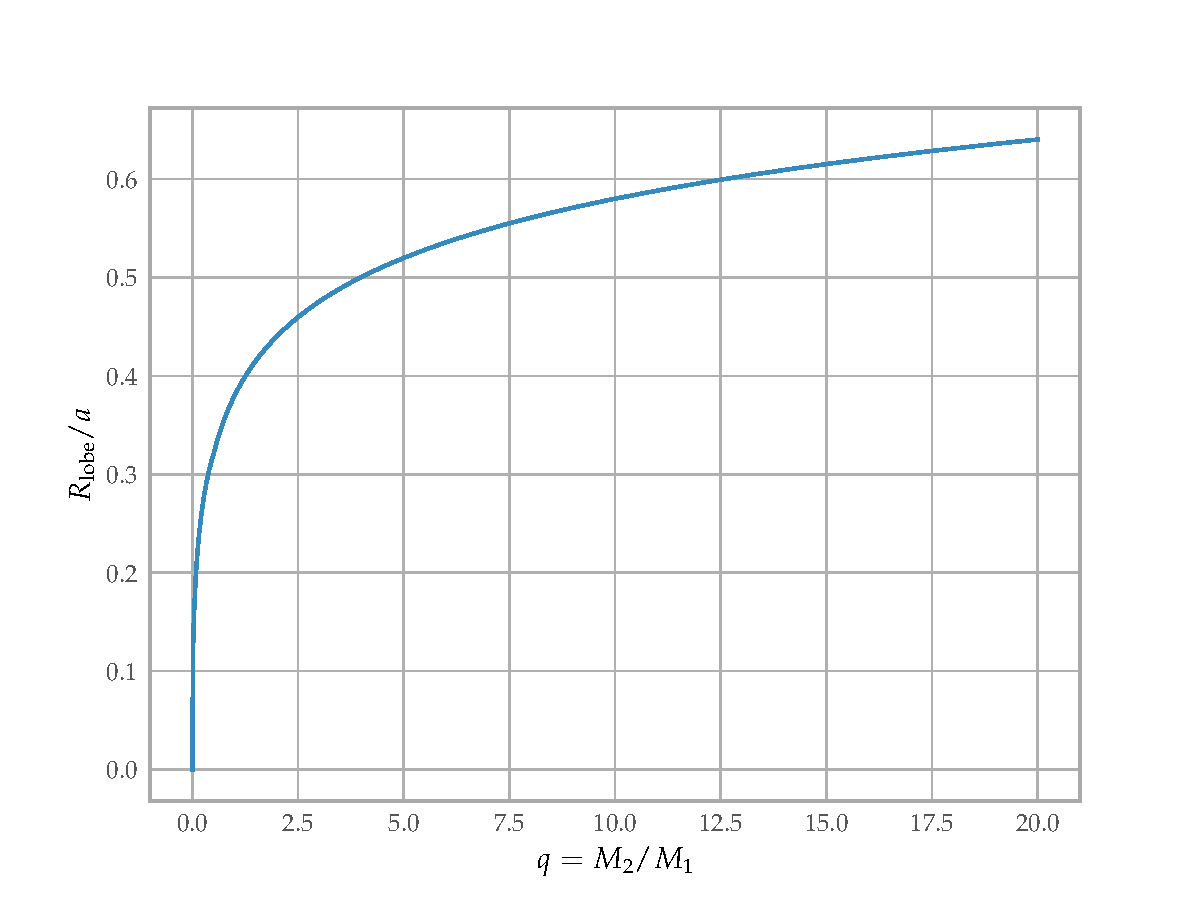
\includegraphics[width=\textwidth]{figures/roche-lobe-radius}
\caption{Radius of the Roche lobe as a function of \(q\).}
\label{fig:roche-lobe-radius}
\end{figure}

However, the orbital separation \(a\) is itself a function of \(q\), and the dependence \(a(q)\) is much more relevant than the dependence of \(R _{\text{lobe}} / a\). 

In order to calculate \(a(q)\), let us make some assumptions. 
\begin{enumerate}
    \item \(M_1 + M_2 = \const\). This is realistic: it is hard for the binary star system as a whole to lose or gain mass.
    \item The total angular momentum \(L _{\text{tot}}\) is a constant. This is a bit tricky: even a small amount of mass loss can result in high angular momentum loss. 
    \item \(L _{\text{tot}} = L _{\text{orb}}\): all the angular momentum is orbital. We are neglecting the spins of the stars, and the angular momentum of the gas. This is realistic, since tidal forces move the configuration towards a tidally locked state. 
\end{enumerate}

The conservation of mass tells us that \(M_1 (1 + q)\) is constant. 
The orbital angular momentum is written in terms of the distances of the stars from the center of mass:
%
\begin{align}
L _{\text{orb}} &= M_1 v_1 a_1 + M_2 v_2 a_2  \\
&= M_1 a_1^2 \omega + M_2 a_2^2 \omega 
\,,
\end{align}
%
so if we place the origin of our coordinates in the center of mass we can write everything in terms of the orbital separation \(a = a_1 + a_2 \):
% \todo[inline]{So \(a\) is not the semimajor axis}
%
\begin{align}
-M_1 a_1 + M_2 a_2 &= 0  \\
- (M_1 + M_2 ) a_1 + M_2 a &= 0  \\
a_1 &= \frac{qa}{1+q} \\
a_2 &= \frac{a}{1 +q}
\,.
\end{align}

In terms of angular momentum we get 
%
\begin{align}
\qty[
    M_1 \frac{q^2 a^2}{(1 + q)^2}
    + M_2 \frac{a^2}{(1+q)^2}
]\omega &= \const \\
M_1 a^2
\qty[
    \frac{q^2}{(1 + q)^2}
    + \frac{q}{(1+q)^2}
]\omega &= \const 
\,,
\end{align}
%
which means 
%
\begin{align}
\frac{a^2 M_1 \omega q}{1 + q} =
\frac{a^2 M_1 2 \pi  q}{P(1 + q)} 
= \const
\,,
\end{align}
%
since \(\omega = 2\pi / P\), where \(P\) is the orbital period. 
We also know that (because of mass conservation) \(M_1 \propto (1 + q)^{-1}\), therefore 
%
\begin{align}
\frac{a^2 q}{(1+q)^2} \frac{1}{P}
\,,
\end{align}
%
but also Kepler's third law tells us that \(a^3 \propto P^2\): so, \(P \propto a^{3/2}\). This yields 
%
\begin{align}
\frac{a^{2 - 3/2} q}{(1+q)^2} = \sqrt{a} \frac{q}{(1+q)^2} = \const
\,,
\end{align}
%
therefore 
%
\begin{align}
a \propto \frac{(1 + q)^{4}}{q^2}
\,.
\end{align}

The Roche lobe \(R_2\) for \(M_2\) is given by \(R_2 = a f\), therefore
%
\begin{align}
\log R_2 = \log a + \log f
\,,
\end{align}
%
and if we consider a variation of \(q\), the variation of \(\log R_2 \) will be given by the sum of the variations of the two logarithms. 

Because of the expression we derived, we have 
%
\begin{align}
\log a &= 4 \log (1 +q) - 2 \log q + \const \\
\Delta \log a &= 4 \frac{\Delta q}{1 + q} - 2 \frac{\Delta q}{q }  \\
&= \frac{4q -2 -2 q}{(1 + q) q} \Delta q = 2 \frac{\Delta q}{q} \frac{q -1}{q +1}
\,.
\end{align}

Then, the fractional variation is approximately 
%
\begin{align}
\frac{\Delta R_2}{R_2} = \Delta \log R_2 \approx 
2\frac{\Delta q}{q} \frac{q -1}{q +1}
\,,
\end{align}
%
since \(\Delta \log f\) is negligible (see figure \ref{fig:roche-lobe-relative-corrections}). 
As the star \(M_2 \) donates mass, \(M_2 \) decreases and \(M_1 \) increases. Then, \(q = M_2 / M_1 \) decreases, therefore \(\Delta q < 0\). 

\begin{figure}[ht]
\centering
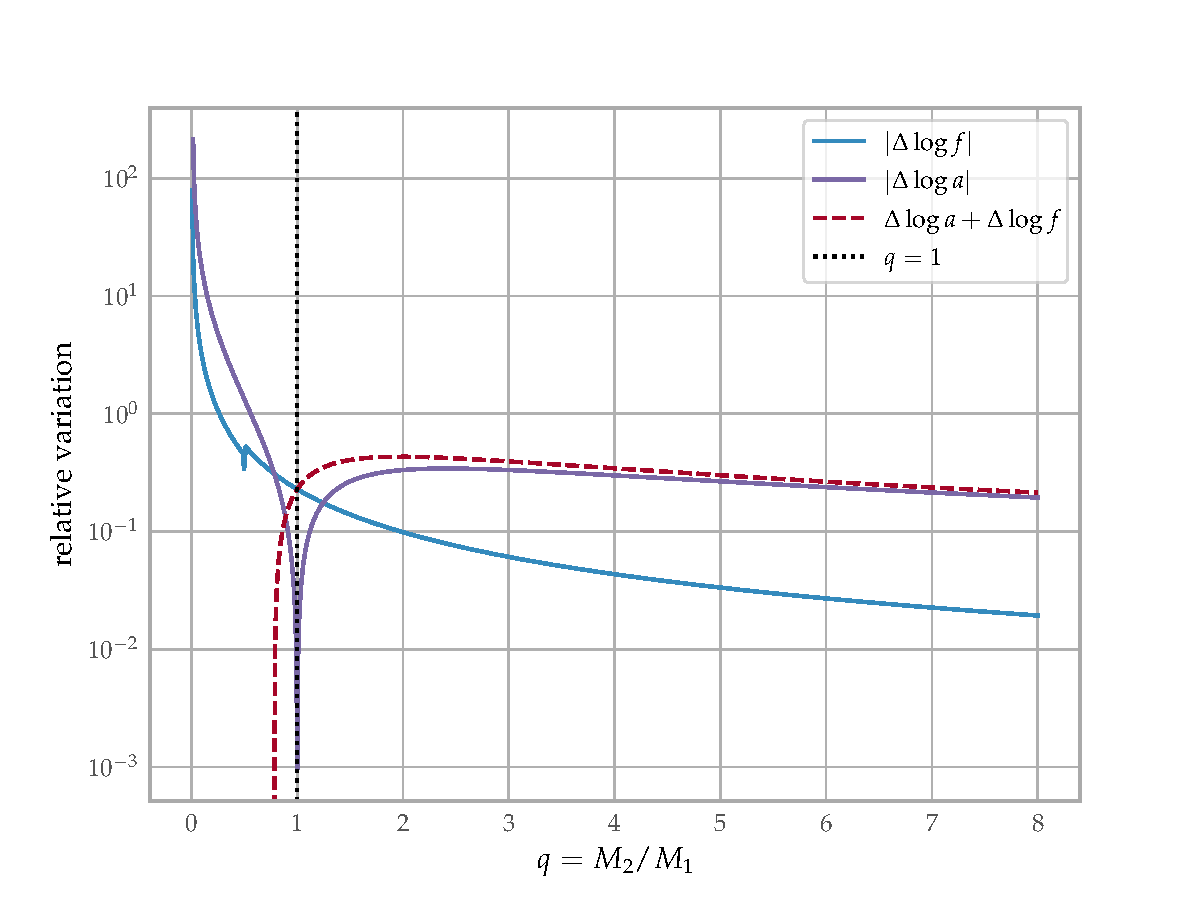
\includegraphics[width=\textwidth]{figures/roche-lobe-relative-corrections.pdf}
\caption{Relative size of the corrections --- \(\Delta \) means derivative with respect to \(q\). One can notice that for typical \(q \gtrsim 2\) the magnitude of \(\Delta \log a\) is about one order of magnitude larger than that of \(\Delta \log f\). Also, we can see that \(\Delta \log a + \Delta \log f\) is indeed positive for \(q > 1\) --- the curve is not shown in the region in which it is negative.}
\label{fig:roche-lobe-relative-corrections}
\end{figure}

If we want the Roche lobe to shrink, we want \(\Delta R_2 < 0\): so, we want \(q - 1 > 0\). 
This means that \textbf{Roche lobe accretion is self-sustaining, or stable iff the donor star is larger than the receiver}. 
% Including \(\Delta f\), things don't change by much. 
If we include \(\Delta f\), as one can see in figure \ref{fig:roche-lobe-relative-corrections}, the picture is quite similar --- the noticeable correction we have is that systems with \(\num{.8} < q < 1\) might still have Roche Lobe Overflow. 

Is this the case in real systems? Usually the mass of the BH is of at least a few solar masses, so we need an unusually large companion. 
For example, the companion to the BH in Cygnus X-1 is a very large O-star. 

\section{Accretion disks}

Now we will discuss what happens when this is indeed the case. What is the fate of the matter passing through the inner Lagrange point? 

Let us change the perspective: we are not comoving with respect to the orbiting stars anymore. 
Let us call \(b_1 \) the separation of the \(L_1 \) point from the center of star 1. This is slightly larger than \(R_1 \). 

If we are stationary at the center the companion compact star will appear to rotate at a large velocity compared to us. 

The components of this velocity can be decomposed into the parallel and perpendicular to the separation vector between the star, however the component \(v _ \parallel\) will be of the order of the speed of sound in the gas: roughly, 
%
\begin{align}
v_{\parallel} \approx c_s = \sqrt{ \pdv{P}{\rho }} = \sqrt{\frac{k_B T}{\mu m_p}} \approx \num{10} \sqrt{ \frac{T}{\SI{e4}{K}}} \SI{}{km /s}
\,;
\end{align}
%
while the component \(v_\perp\) will be large: of the order of 
%
\begin{align}
v_\perp \sim b_1 \omega 
\,,
\end{align}
%
and the distance \(b_1\) will be roughly given by \cite[]{plavecTablesRocheModel1964}
%
\begin{align}
b_1 \approx a (\num{.5} - \num{.227} \log q)
\,,
\end{align}
%
while by Kepler's third law 
%
\begin{align}
4 \pi^2 a^3 = G (M_1 + M_2 ) P^2
\,,
\end{align}
%
so 
%
\begin{align}
a \approx \num{3e11} \qty(\frac{M_1 }{M_{\odot}})^{1/3}
\qty(1 + q)^{1/3}
\qty(\frac{P}{\SI{1}{d}})^{2/3} 
\SI{}{cm}
\,,
\end{align}
%
while the angular velocity is 
%
\begin{align}
\omega = \frac{2 \pi }{P} \approx \num{7e-5} \qty(\frac{P}{\SI{1}{d}})^{-1} \SI{}{rad/s}
\,.
\end{align}

This means that the perpendicular velocity is approximately 
%
\begin{align}
v_{\perp} \approx \num{100} \qty(\frac{M_1 }{M_{\odot}})^{1/3}
\qty(1 + q)^{1/3}
\qty(\frac{P}{\SI{1}{d}})^{-1/3}
\SI{}{km/s}
\,,
\end{align}
%
an order of magnitude more than the speed of sound. 

\end{document}
